%%% Version 3.3 Generated 2016/11/10 %%%
%%% You will need to have the following packages installed: datetime, fmtcount, etoolbox, fcprefix, which are normally inlcuded in WinEdt. %%%
%%% In http://www.ctan.org/ you can find the packages and how to install them, if necessary. %%%
%%%  NB logo1.jpg is required in the path in order to correctly compile front page header %%%

\documentclass[utf8]{frontiersSCNS} % for Science, Engineering and Humanities and Social Sciences articles
%\documentclass[utf8]{frontiersHLTH} % for Health articles
%\documentclass[utf8]{frontiersFPHY} % for Physics and Applied Mathematics and Statistics articles

%\setcitestyle{square} % for Physics and Applied Mathematics and Statistics articles
\usepackage{url,hyperref,lineno,microtype,subcaption}
\usepackage[onehalfspacing]{setspace}

\usepackage{booktabs}
\usepackage{multirow}

\linenumbers


% Leave a blank line between paragraphs instead of using \\


\def\keyFont{\fontsize{8}{11}\helveticabold }
\def\firstAuthorLast{Sample {et~al.}} %use et al only if is more than 1 author
\def\Authors{First Author\,$^{1,*}$, Co-Author\,$^{2}$ and Co-Author\,$^{1,2}$}
% Affiliations should be keyed to the author's name with superscript numbers and be listed as follows: Laboratory, Institute, Department, Organization, City, State abbreviation (USA, Canada, Australia), and Country (without detailed address information such as city zip codes or street names).
% If one of the authors has a change of address, list the new address below the correspondence details using a superscript symbol and use the same symbol to indicate the author in the author list.
\def\Address{$^{1}$Laboratory X, Institute X, Department X, Organization X, City X , State XX (only USA, Canada and Australia), Country X \\
$^{2}$Laboratory X, Institute X, Department X, Organization X, City X , State XX (only USA, Canada and Australia), Country X  }
% The Corresponding Author should be marked with an asterisk
% Provide the exact contact address (this time including street name and city zip code) and email of the corresponding author
\def\corrAuthor{Corresponding Author}

\def\corrEmail{email@uni.edu}




\begin{document}
\onecolumn
\firstpage{1}

\title[Running Title]{Predicting age with machine learning, using synchronized speech and MEG recordings in children} 

\author[\firstAuthorLast ]{\Authors} %This field will be automatically populated
\address{} %This field will be automatically populated
\correspondance{} %This field will be automatically populated
 
\extraAuth{}% If there are more than 1 corresponding author, comment this line and uncomment the next one.
%\extraAuth{corresponding Author2 \\ Laboratory X2, Institute X2, Department X2, Organization X2, Street X2, City X2 , State XX2 (only USA, Canada and Australia), Zip Code2, X2 Country X2, email2@uni2.edu}


\maketitle


\begin{abstract}

%%% Leave the Abstract empty if your article does not require one, please see the Summary Table for full details.
\section{}
For full guidelines regarding your manuscript please refer to \href{http://www.frontiersin.org/about/AuthorGuidelines}{Author Guidelines}.

As a primary goal, the abstract should render the general significance and conceptual advance of the work clearly accessible to a broad readership. References should not be cited in the abstract. Leave the Abstract empty if your article does not require one, please see \href{http://www.frontiersin.org/about/AuthorGuidelines#SummaryTable}{Summary Table} for details according to article type.

\begin{itemize}
\item Talk about dataset
\item Regression on age with multi-modal dataset + main result
\item Compare feature based classification + results and Augmented raw/real data +results
\item Should also specifically mention added a novel augmentation system
\end{itemize}


\tiny
 \keyFont{ \section{Keywords:} Deep Learning, Machine Learning, Convolutional Neural Networkds, MEG, Language Acquisition, Brain Computer Interface, Data Augmentation}
\end{abstract} 

\section{Introduction}

% Opening is pretty cliche

Machine learning (ML) and in particular deep learning have become an invaluable tool for the medical community in a broad sense. It is being used for DNA stuff \cite{}, learning clusters... ML has also been applied with varying success to classify and interpret brain activity recorded in the form of magnetoencephalography (MEG), electroencephalogrophy (EEG) and functional magnetic resonance imaging (fMRI).

Here we present work that tries to improve the efficacy of machine learning as a tool for classifying MEG (and utltimately other related brain recording) data. This effort is towards ML's use as a better anlysis tool and more accurate system for brain-computer interfaces (BCI). We focus on a dataset of MEG recordings of children performing speech elicitation tasks and synchronized Audio recording. We first compare the predictive ability of the MEG and Audio datasets performing a regression task, then work towards an end-to-end classification approach, including the use of data-augmentation as a way to enable deep learning style models that would otherwise require extremely large datasets. We contrast their efficacy at prediction and analyze the parameters the models develop for any revealing insights. Previous work using MEG and various ML techniques includes detecting hand movement \cite{Asano2009}, identifying schizophrenia \cite{Ince2008}, and on discriminating between sets of imagined words \cite{Guimaraes2007}. To classify between three different hand movements\footnote{Corresponding to the signs in the game of `rock, paper, scissors'.}, Asano {\em et al.} \cite{Asano2009} used an adaptive spatial filter, principal components analysis (PCA) and a support vector machine (SVM) to achieve 62.6\% on held-out test data. In Ince {\em et al.} \cite{Ince2008}, a subject performed a working memory functional task while MEG data were recorded; an SVM with recursive feature elimination (SVM-RFE) was then used to both select a concise feature set and to identify schizophrenia. SVM-RFE recursively discarded features that did not significantly contribute to the margin of the SVM classifier to prevent excessive overfitting on the training set, and achieved 83.8\% to 91.9\% on the test data.

Similar work focusing on speech generation using ML include: Guimaraes {\em et al.} \cite{Guimaraes2007} who classified sets of 7-9 imagined words in two subtasks. In the first, the subject was simply required to attentively listen to a spoken word, while in the second the subject was shown each word visually and told to recite it silently. Those data were then examined using linear discriminant classification and SVM algorithms to classify each channel, and further analyzed in terms of the effects of spatial PCA, independent components analysis (ICA) and second-order blind identification decomposition. By combining channels, Guimaraes {\em et al.} achieved 60.1\% mean classification rate on nine auditory words and 97.5\% maximum mean classification rate on two-word problems.

These works all typically focus on a multi-stage approach to developing a ML classifier which we loosely term as a \emph{feature based approach}. First data is collected and preprocessed using a variety of techniques, \emph{eg.} cropping, trial averaging, normalization, band-pass filtering, linear transforms such as principle component analysis (PCA) and independent component analysis (ICA), and in some cases a spatial filters such as common spatial patterns (CSP) are used (CSP in particular has shown some success in the case of detecting movement-related activity \cite{Schirrmeister2017}). The goal of the preprocessing stage is to overcome the low signal to noise ratio typical of these types of recordings which make training models very difficult and is generally a necessity across most neuroscientific data. Next \emph{features} are calculated from this data, taking a variety of forms, but most commonly employ spectral characteristics in the canonical activity bands (alpha, beta, etc.)\cite{} and statistical moments \cite{}. Finally these features and their associated labels (when performing \emph{supervised} classification) are used to train a ML model which can range from... The advantage of this approach is that expert knowledge about the data can help circumvent the poor signal quality and encourage ML models to distinguish between classes using established signal correlates. The other face of this advantage is the \emph{requirement} of expert knowledge, and the underlying assumptions it may reinforce. Additionally this approach can obfuscate the valuable insights that the ML models may reveal, in the sense that successful ML models (and in particular hierarchical deep models) learn hierarchical representations of data that . Thus an end-to-end approach with nearly raw signal inputs could prove a valuable analytical tool in addition to easing the development of BCIs.

We define an end-to-end approach as training a ML model with raw data that has had minimal to no preprocessing applied to it all. Previous work in end-to-end training using brain signals and modern deep learning techniques include: Schirrmeister {\em et al.} \cite{Schirrmeister2017}, who show an improvement over the previous state of the art implementation with their best models. They consider two layer convolutional networks in a configuration that can simulate filter bank common spatial patterns (FBCSP), five layer deep convolutional networks and residual networks to classify movement on the publically available BCI computition IV dataset 2a \cite{}. Furthermore they employ a basic data augmentation technique of a sliding window cropping strategy that improves the performance of their models. We are unaware of any such work using MEG recordings.


% Need to transition to the age/speech context before using a version of this paragraph

Talk about how we could select features by hand, based on previous work?

For example, Doesburg {\em et al.} \cite{Doesburg2016} predict language ability as an increase in network synchrony with the increase of age during verb-generation (VG) tasks in children and adolescents. They observed a significant increase in the number of synchronous regions with older adolescents, compared with younger children. Furthermore, Yu {\em et al.} \cite{Yu2014} noticed distinct profiles of de-synchrony in VG tasks for children within five age ranges (i.e., 4-6, 7-9, 10-12, 13-15, and 16-18 years of age). These findings indicate the possibility of inferring a child's age from observed MEG data, provided the ability to convey synchronicity and coordinated activity.
Previous work with electroencephalpgraphic (EEG) experiments use common spectral features such as the fast Fourier transform (FFT) magnitude and signal energy within consequetive time windows and various classifiers to accurately differentiating different persons \cite{Nguyen2012, Poulos2001}, and thus may represent synchronicity information. 



% This hypothesis might not be relevant in the more exploratory perspective now presented 
%% We hypothesized that the accuracy of a regression model trained using a combined dataset of MEG and audio features would be greater than that of models trained with only audio and MEG respectively. We postulated that this would be due to the fact that extracting features from time-windowed MEG data would represent information about synchronicity and activity localization that would not otherwise be apparent with speech alone.

\section{Data}

These data were originally recorded for work on age- and sex-related developmental language differences by Doesburg \emph{et al.} and Yu \emph{et al.} \cite{Doesburg2016, Yu2014}. Table \ref{tab:subjects} summarizes some participant demographics. Each participant spoke English as their first language and had no known or suspected histories of speech, language, hearing, or developmental disorders, according to their parents. Prior to the experiment, children received two standardized clinical tests: the Peabody Picture Vocabulary Test (PPVT) \cite{Dunn97} and the Expressive Vocabulary Test (EVT) \cite{EVT}. All children's scores were at or above expected scores for their ages on the PPVT and EVT, and their speech showed neither signs of articulatory difficulties nor any significant effect of age, as visualized in Figure \ref{fig:ppvtevt}. In total, 80 participants were right-handed, 5 were left-handed, and 7 were ambidextrous, according to the Edinburgh assessment; there is no significant variation of handedness with age.

%% \begin{figure}
%% \includegraphics[width=\columnwidth]{PPVTEVT.pdf}
%% \caption{Normalized PPVT and EVT scores across ages for all participants. There are neither signs of speech production impairment nor effect of age on these assessments.}
%% \label{fig:ppvtevt}
%% \end{figure}

Three distinct speech-elicitation stimuli were used. The first two were of the monosyllable /{\em pah}/ and the multisyllabic sequence /{\em pah tah kah}/, respectively. These were simple enough for young children and are part of the diadochokinetic rate (DDK) test, which can be used to evaluate neuromuscular control in motor speech disorders. The incisive nature of these stimuli for measuring speech production make them ideal for this study. Prior to acquisition, the experimenter demonstrated the productions of each stimuli, without word-like prosodic patterns. The third experiment was an overt verb generation (VG) task in English, where subjects are presented with an image they are familiar with, and are asked to produce a verb associated with the object \cite{Doesburg2016}.

Recordings were made in a sound-proof room, with each participant lying supine in a magnetically shielded room in the Neuromagnetic Lab of the Hospital for Sick Children in Toronto, using a CTF whole-head MEG system (MEG International Services Ltd., Coquitlam, BC, Canada). The system recorded all 151 MEG channels, and a single audio channel, with a sampling rate of 4 kHz.

\section{Methods}

%Overview of experiments, data processing and analysis performed

\subsection{Data processing}


We resampled MEG signals at 200 Hz, and band-pass filter between 0.5 Hz and 100 Hz, to remove offsets and accommodate the canonical ranges of delta, theta, alpha, beta, and gamma activity. Electro-ocular (EOG) artifacts were removed using automated blind source separation (BSS), and measure signal complexities using fractal dimensions. Auto-BSS filters EOG artifacts using the SOBI algorithm in AAR's implementation \cite{eog}. This preprocessing step was common to our feature-based and end-to end approaches, as we deemed it a minimal necessary steps.

To further preprocess our data to develop our feature based datasets we applied info-max independent component analysis (ICA) \cite{Bell1995} to determine statistically independent sub-components of the MEG recordings, across all subjects. This was done by appending MEG recordings for all subjects into a single 151-channel matrix for each of the 3 speech-elicitations: /{\em pah}/, /{\em pah tah kah}/ and the VG task performed using the EEGLAB toolbox \cite{Delorme04eeglab}. We then apply the resulting sphering and weight matrices, determined by ICA for each test condition, to each subject's respective recordings. These recordings (i.e., both MEG and audio separately) are then separated into windowed epochs corresponding to $-500$ ms to $+1500$ ms frames around the onset of the stimuli prompt.

\subsection{Feature extraction}

We extracted a total of 156 acoustic features and 4681 MEG features from each epoch using openSMILE \cite{Eyben13-RDI}. These are calculated using 50 ms rectangular windows, with a 25 ms overlap of the previous window for each successive window, resulting in a total of 79 windows per datapoint.

\subsubsection{Audio features}

Features to represent spectral activity are calculated, for each window, using both a 128-point fast Fourier transform and linear predictive coding coefficients. Additionally, the statistical moments, mean (also absolute mean, quadratic mean, and aforementioned means calculated using only non-zero values), variance, skewness and kurtosis are calculated. Finally, the root-mean-squared and log of the signal energy are also calculated for each window.

\subsubsection{MEG features}

We extract 31 features for each of the 151 independent components derived from the MEG data. These consist of an 8-point fast Fourier transform, statistical moments, and energy calculation identical to the audio signal, and the autocorrelation function (ACF) calculated using the fast Fourier transform (FFT) and its inverse (iFFT) for window $w$:

% Probably could use some more discussion of the features here?

\begin{equation}
  ACF(w) = iFFT(|FFT(w)|^2)
  \label{eq1}
\end{equation}

\subsection{Sensor Projection}

To better represent the spatial structure of the recordings, we perform some experiments using a series of image representations of the data. The data is nominally saved in a 2-dimensional array whose first dimension corresponds to samples in time, and second dimension is of length 151 corresponding to the 151 MEG channels in no spatially significant ordering. To represent the spatial nature of the data, the locations of the 151 channels of the MEG sensor array for each experiment are projected using an azimuthal projection on to a two-dimensional grid sized $100 \times 100$, and then the raw values of each sensor are  interpolated based on the nearest (projected) sensor accross this grid to generate a series of images, \emph{ie.} a three dimensional with dimensions $samples \times  100 \times 100$. A similar approach was used in \cite{}, where EEG data was projected and then interpolated into a series of images, but instead of using raw data as we do here, they create multiple channels (as one would have with multiple colour channels) which represented different spectral features (in their case the X, Y, and Z frequency bands). We chose not to take this approach, as this first of all increased the dimensionality of the problem immensely and, as it was implemented in \cite{}, the multiple-features-as-channels required a strong assumption of which spectral band the distinguishing data will appear to keep the number of channels down, which is to some degree not in the spirit of end-to-end learning.

\subsection{Data Augmentation}

To help facilitate end-to-end learning, we employed three techniqes that would produce multiple usable training points from the same recordings. There are many 

\subsubsection{Cropping}

Here fixed length crops of the entire recording are taken such that the event of a trial is localized in a different place for each augmented data point. Effectively, rather than one training datapoint for each trial performed, a sliding window smaller than the length of the trial is used to crop many individual points. The premise behind this augmentation is that with the event localized in different places, an architecture like a CNN learns temporal filters that are agnostic of any specific point in time. Although ideally when using gradient based training, the training points are independent and identically distributed (I.I.D) \cite{}, augmentation such as this 

\subsubsection{Subsampling}

We take advantage of the high sampling rate of the recordings ($4kHz$) being used with respect to the frequency ranges that that we keep  for analysis and examine whether different sub-sampling of the data is a viable augmentation strategy. Filtering is still applied as before to minimize aliasing artifacts, and then we augment the number of samples by re-sampling at a frequency of $200 Hz$

\subsubsection{Noisy Sensors}

To the authors' knowledge, the only other attempt at performing some sort of spatial augmentation for this type of data is presented in \cite{}. Here they...


\subsection{Data analysis}

First, we identify correlations among extracted features, in order to demonstrate evidence for predictive potential. We then train regularized multilinear regression models to predict a subject's age.

All regression and classification models are evaluated using the same held out test subjects, using ten-fold cross-validation. The test set has a nearly identical distribution of age

\subsubsection{Correlation}

We used standard Pearson correlation between the extracted MEG and audio features, for each experiment set separately. We set significance for $p$-values at $\alpha = 10^{-4}$ and the coefficient $r$'s absolute value $\text{abs}(r) > 0.2$. For each experiment, we then examined the independent component that had the highest correlations of its features with respect to audio features, to determine if there were any noticeably consistent brain locations that were being emphasized. These are plotted in figure \ref{fig:components}. Furthermore, we compute correlation of MEG and audio features, with respect to age, over the entire data set, to identify features with a potentially stronger predictive capability for regression.

\subsection{Trained Models}

\subsubsection{Multilinear regression}

We train multilinear regression models to predict age using each of the \textit{Audio}, \textit{MEG}, and the fused \textit{Audio+MEG} datasets respectively. We use 10-fold cross-validation within each dataset. The test and training sets are selected to have a similar mean and standard deviation over the ages of participants. We perform Bayesian parameter optimization using Hyperopt \cite{Bergstra2013} on the first fold of data to determine an appropriate learning rate and regularization factor for all training.

Since the number of features multiplied by the number of time windows exceeds the total number of data points available to train, we reduce the dimensionality of the MEG data (i.e., {\em MEG (red.)}) by selecting only those features from that set that have significant correlations, as defined above.

\subsubsection{Logistic Regression and Linear Support Vector Machine}

These are commonly used classifiers that learn linear (although they can be modified to create non-linear) separatations between the points of output classes. The main difference between the two is that logistic regression (or softmax classifier) maximizes the confidence of the prediction by..., whereas as a linear support vector machine, or SVM . Here in particular we use an L2 regularized SVM or L2-SVM

\subsubsection{Multi-Layer Perceptron}

This is the most straight-forward implementation of a neural-network classifier. It is also known as a feed-forward neual network. It consists of a number of layers of neurons, where typically less than three layers are considered shallow, but with three or more the literature starts to call them \textit{deep}. Each neuron recieves input from each of the neurons of the previous layers, with the first layer recieving the entire input. These incoming ``connections'' are weighted, and these weights are trained to fit the dataset using gradient descent (in addition to other optimization techniques like \cite{adam, rmsprop, etc}). Crucially the output of each neuron has a non-linear operation applied to the weighted sum of all incoming connections. This applies for the most part all neural network implementations, and allows them to learn arbitrary functions that seperate output labels.

\subsubsection{Convolutional Neural Network}

A convolutional neural network is a variation on the feed-forward neural network that employs the sharing of incoming weights for the purpose of both reducing the number of parameters, and learning convolution-like operations, rather than the feed-forward networks masking based operations.

\subsubsection{Recurrent Neural Network}

\section{Results}

\subsection{Correlations}

\subsubsection{MEG vs. audio: /pah/}

Only $0.0163$\% of the $156 \times 4681$ correlations are significant after correction, on these data. Therefore, there appears to be little redundancy between the MEG and Audio features analyzed, which supports the rationale for their combined analysis. Of these significant correlations, all were with respect to three audio features. These features corresponded to sequential FFT bins that represent the frequency range 340-400 Hz. The most correlated MEG feature is the autocorrelation measure for six different independent components.

\subsubsection{MEG vs. audio: /pah tah kah/}

Under this test condition, $0.0116$\% of correlations between features are significant and, similar to the /{\em pah}/ stimuli, these correlations heavily involve the audio features that represent frequencies 320-400 Hz, in addition to some features that represent much lower frequencies 80-160 Hz, which may be due to noise in the environment. Also similar to the /{\em pah}/ experiment, the autocorrelation feature seems to be significantly correlated for 8 components, three of which are the same components as the /{\em pah}/ stimuli.

% The frequency range 340-400 pops up both times, it seems to be too low to be related to formats or F0, but I can't say for sure because for some reason I commented out the formants section of my opensmile configuration, I calculate the LPC anyway, but I didn't even leave myself a note as to why I did that...

\subsubsection{MEG vs. audio: Verb Generation}

When considering this test set, $0.132$\% of correlations between features are significant, which is a somewhat substantial increase relative to the previous two correlation comparisons. Similar to the above correlations, autocorrelations and spectral activity appear prominantly, in addition to mean and energy features. 

\begin{figure}[t]
  \centering
  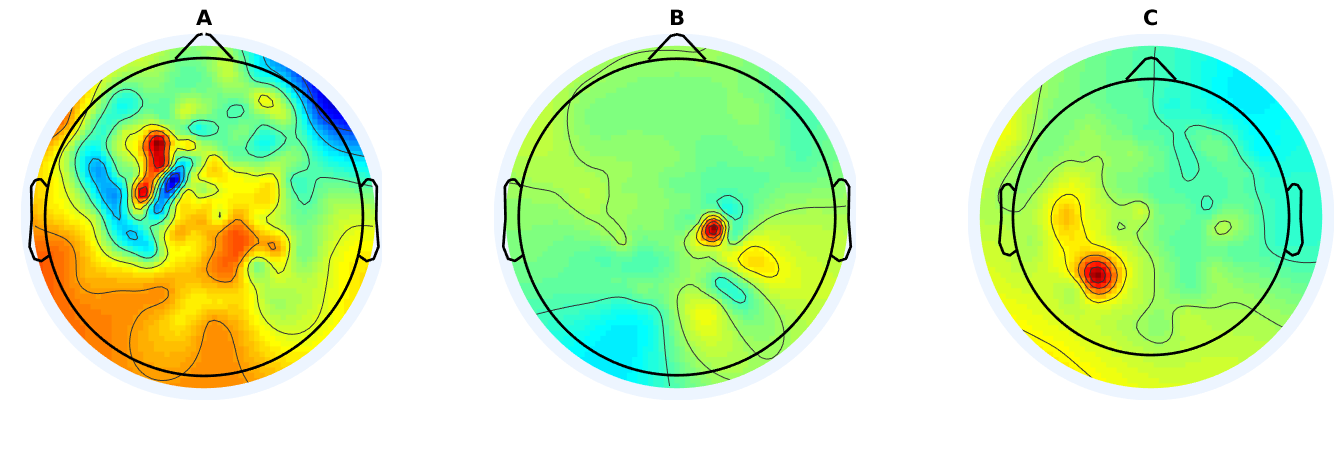
\includegraphics[width=\linewidth]{AllComponents.png}
  \caption{Graphical illustrations (using \cite{Delorme04eeglab}) of the independent components with features most correlated with audio features, from left to right, /{\em pah}/, /{\em pah tah kah}/ and verb generation experiments. These are generated using the ICA weight matrix interpolated over MEG sensor locations. }
  \label{fig:components}
\end{figure}
 
\subsubsection{All features vs. age}

When correlating with age, 172 features were found to have significant values, all of which were MEG features. This includes the autocorrelation features of eight (ICA) components -- including the first (highest entropy) component -- in addition to the entire available frequency spectrum of four of these components and one other. The fact that spectral features are relatively strongly correlated with age might provide evidence that synchronization may be a distinguishing factor across age, but additional feature analysis will be necessary to confirm this.

The correlation of a single computed component has correlation coefficients $\text{abs}(r)>0.3$ for nearly all of its features, which was true of no other components considered. Examining the physical representation of these components with respect to each of the three experiments, there were no discernible similarities to note. Three other components also had features with correlation $\text{abs}(r)>0.3$, for features that corresponded to various mean variants.

\subsection{Regression}

\begin{table}[t]
  \centering
  \label{tab:reg_results}
  \begin{tabular}{| l | c | c |}
    \toprule
    \multicolumn{1}{l}{\textbf{Feature set}} & \multicolumn{1}{c}{\textbf{Mean}} & \multicolumn{1}{c}{\textbf{Variance}} \\
    \toprule
        Audio~~~                             & ~~~$4.103$         &     $0.473$       \\
        MEG~~~                               & ~~~$4.896$         &     $0.234$       \\
        Audio+MEG~~~                         & ~~~$4.109$         &     $0.244$       \\

        \midrule
       
        MEG (red.)~~~                        & ~~~$5.081$         &     \textbf{0.142}       \\
        Audio+MEG (red.)~~~                  & ~~~\textbf{3.370}         &     $0.248$       \\

        \bottomrule
  \end{tabular}
  \caption{Root mean squared error (RMSE), in years, of 10-fold cross validation for each of the feature sets. Audio features combined with reduced MEG features show the best prediction capability. Bold indicates best performance.}
\end{table}

The regression performance across the 10 folds seems to suggest that a multilinear regression model trained using both audio and the reduced (i.e., highly correlated) MEG feature sets performs better than either Audio or MEG feature sets alone. Without  reducing the MEG feature set, regression performance is no better than that for Audio alone. Models trained using some MEG features also  perform more consistently (i.e., with lower variance) than with Audio features exclusively.

When trained using the highly correlated MEG features, regression performance is nearly equivalent to its exhaustive counterpart. There is a fairly marked reduction in variance, but performance does not increase until Audio and MEG features are combined. This may be surprising, considering that the MEG features are relatively correlated with age. This could suggest somewhat complementary information between data sets. % FR: in future, a measure of mutual information should be computed.

Table \ref{tab:reg_results} shows the means and variances of root mean squared error (RMSE) values on regression, given various combinations of feature sets. Clearly, combining audio features with a reduced set of MEG features result in the best accuracy on average. An $n$-way ANOVA confirms a significant effect of the feature type on regression accuracy ($F_{4,49} = 51.05$, $p<0.001$), with the combined Audio + reduced MEG features being significantly more accurate than {\em each} of the other combinations, according to right-tailed $t$-tests, after correcting $\alpha$, with Bonferroni, for multiple comparisons.

\subsection{Feature Based Classification}

\begin{table}[t]
  \centering
  \label{tab:feat_results}
  \begin{tabular}{l l | c | c}
    \textbf{Feature set} & Model & \textbf{Mean \%} & \textbf{Variance \%} \\
    \toprule
    \multirow{3}{*}{Audio}
    & Logistic Regression & 25.3 & 3.20  \\
    & Linear SVM          & NaN & NaN  \\
    & Shallow NN          & 44.7 & 1.33  \\
    \midrule
    \multirow{3}{*}{MEG}
    & Logistic Regression & 44.4 & 10.9  \\
    & Linear SVM          & NaN & NaN  \\
    & Shallow NN          & NaN & NaN  \\
    \midrule
    \multirow{3}{*}{Audio + MEG}
    & Logistic Regression & 14.0 & 1.14  \\
    & Linear SVM          & NaN & NaN  \\
    & Shallow NN          & 64.0 & 5.03  \\
    \bottomrule
  \end{tabular}
  \caption{Classification accuracy using one of three datasets, and three different basic classifier models.}
\end{table}

We found very little success in training the recurrent neural networks using the feature based datasets, furthermore the addition of attention made no sugnificant improvement 
  

\subsection{End-to-End Classification}

\begin{table}[t]
  \centering
  \label{tab:end2end_results}
  \begin{tabular}{l l | c | c}
    \textbf{Feature set} & Model & \textbf{Mean \%} & \textbf{Variance \%} \\
    \toprule
    \multirow{3}{*}{No Augmentation}
    & Logistic Regression & NaN & Nan  \\
    & Linear SVM          & NaN & NaN  \\
    & Shallow NN          & NaN & NaN  \\
    \midrule

    \bottomrule
  \end{tabular}
  \caption{Classification accuracy using real data input under different augmentation strategies and models.}
\end{table}

\section{Discussion}

%% Taken from IS paper, still needs to be changed

This work is a preliminary combination and comparison of aligned Audio and MEG data, in a few speech production tasks, across children of various ages. While there exist relatively few correlations {\em across} these modalities -- and those that exist are relatively low -- they both provide similarly informative predictive power towards age regression, and even more so when combined.

To compare with the `optimal' reduced set of features, according to absolute correlation {\em and} their $p$-values, we also {\em randomly} extract a subset of 172 features. Performing multilinear regression on this random selection of features remains insignificantly different than using all features. Finally, we also considered a set of the 172 most correlated MEG features {\em among those} with $p \geq 0.0001$, which accounts for high, but potentially quite variable, correlations. Surprisingly, this improved accuracy slightly on average over using all features, but with a much larger variance (i.e., $\geq 0.9$). The optimum solution remains to force $p<0.0001$ for each correlation. These {\em ad hoc} analyses seem to suggest that increases in performance depend not on merely reducing dimensionality blindly, but on selecting {\em consistently} correlating features.

Performing ICA separately for each stimulus results in different components, naturally. In other words, component $c_i$ with respect to the /{\em pah}/ data is different than component $c_i'$ with respect to the VG data. Future work should consider the sensitivity of any analysis to the stimulus, and be able to generalize ICA analyses that were performed on slightly different data sets.

Audio frequencies just below 400 Hz often correlate with MEG features. For the /{\em pah}/ and /{\em pah tah kah}/ stimuli, our initial hypothesis was that these would relate to F0, or the formant structure of the phone /{\em ah}/. However, whether this is the case remains to be determined.

%\FR{some 'extra' regression analysis can go here -- but main stuff goes in section 4}
% We don't need separate Conclusion and Discussion sections.
%We show a mild confirmation of our hypothesis.

This paper provides a strong baseline indicating that MEG data can provide a significant improvement to age detection, over Audio features alone. We are currently considering more complex models that relate MEG and audio features in conjunction with other features. Although this dataset is relatively large, considering the population and equipment, it will be important to evaluate whether it is sufficiently large to train modern regularized methods in deep learning.

\section{Acknowledgements}

We thank Rui Janson for his help performing automated EOG removal.


\bibliographystyle{IEEEtran/bibtex/IEEEtran}


\bibliographystyle{frontiersinSCNS_ENG_HUMS} % for Science, Engineering and Humanities and Social Sciences articles, for Humanities and Social Sciences articles please include page numbers in the in-text citations
%\bibliographystyle{frontiersinHLTH&FPHY} % for Health, Physics and Mathematics articles
\bibliography{test}

\end{document}
